\documentclass[12pt,t]{beamer}
\usepackage{graphicx}
\usepackage[vlined]{algorithm2e}
\usepackage{times}
\usepackage{calc}
\usepackage{url}
\usepackage{soul}
\usepackage{graphicx}
\usepackage{multirow, hhline}
\usepackage{array, booktabs}
\usepackage{amsmath}
\usepackage{amssymb}
\usepackage{relsize}
\usepackage{multirow}
\usepackage{booktabs}
\usepackage{pagecolor}
\usepackage{lipsum}
\usepackage{capt-of}
\usepackage{booktabs}

\usepackage{graphicx}
\usepackage{multicol}
\usepackage[T1]{fontenc}
\usepackage{ae}
\graphicspath{{fig/}}
\setbeameroption{hide notes}
\setbeamertemplate{note page}[plain]

\usetheme{default}
\beamertemplatenavigationsymbolsempty
\hypersetup{pdfpagemode=UseNone}

\usefonttheme{professionalfonts}
\usefonttheme{serif}
\usepackage{fontspec}
\setmainfont{Karla}
\setbeamerfont{note page}{family*=pplx,size=\footnotesize} % Palatino for notes

\definecolor{foreground}{RGB}{70,70,70}
\definecolor{background}{RGB}{249, 249, 249} %24,24,24
%\definecolor{title}{RGB}{107,174,214} %107,174,214
\definecolor{title}{RGB}{70,70,70}
\definecolor{gray}{RGB}{0,0,0}
\definecolor{subtitle}{RGB}{70,70,70}
\definecolor{hilight}{RGB}{102,255,204}
\definecolor{vhilight}{RGB}{255,111,207}

\setbeamercolor{titlelike}{fg=title}
\setbeamercolor{subtitle}{fg=subtitle}
\setbeamercolor{institute}{fg=gray}
\setbeamercolor{normal text}{fg=foreground,bg=background}


\setbeamercolor{item}{fg=foreground} % color of bullets
\setbeamercolor{subitem}{fg=gray}
\setbeamercolor{itemize/enumerate subbody}{fg=gray}
\setbeamertemplate{itemize subitem}{{\textendash}}
\setbeamerfont{itemize/enumerate subbody}{size=\footnotesize}
\setbeamerfont{itemize/enumerate subitem}{size=\footnotesize}

\setbeamercolor{block title}{fg=white,bg=gray!70}
\setbeamercolor{block body}{fg=black,bg=gray!10}
\setbeamercolor{block title alerted}{fg=red,bg=gray!40}
\setbeamercolor{block title example}{fg=black,bg=green!20}
\setbeamercolor{block body example}{fg=black,bg=green!5}
\setbeamerfont{block title}{series=\bfseries}

\hypersetup{colorlinks,linkcolor=foreground,urlcolor=foreground}


\setbeamertemplate{footline}{%
    \raisebox{5pt}{\makebox[\paperwidth]{\hfill\makebox[20pt]{\color{gray}
          \scriptsize\insertframenumber}}}\hspace*{5pt}}

\addtobeamertemplate{note page}{\setlength{\parskip}{12pt}}


\newcommand{\bi}{\begin{itemize}}
\newcommand{\ei}{\end{itemize}}
\newcommand{\ig}{\includegraphics}
\newcommand{\subt}[1]{{\footnotesize \color{subtitle} {#1}}}

\let\emph\relax % there's no \RedeclareTextFontCommand
\DeclareTextFontCommand{\emph}{\bfseries\em}


\setbeamertemplate{frametitle}
{\vskip4pt
  \leavevmode
%\hbox{%
\begin{beamercolorbox}[wd=\paperwidth,ht=2ex,dp=0ex]{frametitle}%
\underline{\makebox[\paperwidth][l]{\hspace*{10pt}
\large {{\insertframetitle}}}}
\end{beamercolorbox}
%  }%
}

%\setbeamercolor{frametitle}{fg=yellow,bg=red}

\begin{document}

\AtBeginSection[]{
  \begin{frame}
  \vfill
  \centering
  \begin{beamercolorbox}[sep=8pt,center,shadow=true,rounded=true]{title}
    \underline{\makebox[0.8\paperwidth][l]{
\large {{\insertsectionhead}}}}
  \end{beamercolorbox}
  \vfill
  \end{frame}
}

\title{\large{Lecture \#5: Regularization}}
\subtitle{CS 109A, STAT 121A, AC 209A: Data Science}
\author{Pavlos Protopapas \and Kevin Rader}
%\institute{Harvard University}
\date{}
\titlegraphic{
   
\includegraphics[height=2cm]{iacs}
\includegraphics[height=2cm]{hogwarts}
}
{
\setbeamertemplate{footline}{} % no page number here
\frame{
  \titlepage
  
}
}


\begin{frame}{Lecture Outline}
\tableofcontents
\end{frame}

%%%%%%%%%%%%%%%%%%%%%%%%%%%%%%%%%%%%%%%%%%%%%%%%%%%%%%%%%%%%%%%%%%%%%%%%%%%%%%
\section{Review}

%%%%%%%%%%%%%%
\begin{frame}{Model Selection} 
\emph{Model selection} is the application of a principled method to determine the complexity of the model, e.g. choosing a subset of predictors, choosing the degree of the polynomial model etc.
\vskip0.2cm
A strong motivation for performing model selection is to avoid overfitting, which we saw can happen when
\vskip0.4cm
\begin{itemize}
\item there are too many predictors:
\begin{itemize}
\item the feature space has high dimensionality
\item the polynomial degree is too high
\item too many cross terms are considered
\end{itemize}
\item the coefficients values are too extreme
\end{itemize}
\end{frame}

%%%%%%%%%%%%%%
\begin{frame}{Stepwise Variable Selection and Cross Validation} 

Last time, we addressed the issue of selecting optimal subsets of predictors (including choosing the degree of polynomial models) through:
\vskip0.2cm
\begin{itemize}
\item stepwise variable selection - iteratively building an optimal subset of predictors by optimizing a fixed model evaluation metric each time,
\vskip0.2cm
\item cross validation - selecting an optimal model by evaluating each model on multiple validation sets.
\end{itemize}
\vskip0.2cm
Today, we will address the issue of discouraging extreme values in model parameters.
\end{frame}

%%%%%%%%%%%%%%%%%%%%%%%%%%%%%%%%%%%%%%%%%%%%%%%%%%%%%%%%%%%%%%%%%%%%%%%%%%%%%%
\section{Behind Ordinary Lease Squares, AIC, BIC}

%%%%%%%%%%%%%%
\begin{frame}{Likelihood Functions} 
\vskip-0.4cm
\only<1>{
We've been using AIC/BIC to evaluate the explanatory powers of models, and we've been using the following formulae to calculate these criteria
\begin{align*}
\mathrm{AIC} &\approx n \cdot \ln(\mathrm{RSS}/n) + 2 J\\
\mathrm{BIC} &\approx n \cdot \ln(\mathrm{RSS}/n) + J\cdot \ln(n)
\end{align*}
where $J$ is the number of predictors in model.
\vskip0.2cm
Intuitively, AIC/BIC is a loss function that depends both on the predictive error, RSS, and the complexity of the model. We see that we prefer a model with few parameters and low RSS.
\vskip0.2cm 
But why do the formulae look this way - what is the justification?
}
\only<2>{
\footnotesize
Recall that our statistical model for linear regression in vector notation is
\[
y = \beta_0 + \sum^J_{j=1} \beta_i x_i + \epsilon = \pmb{\beta}^\top \pmb{x} + \epsilon.
\]
It is standard to suppose that $\epsilon \sim \mathcal{N}(0, \sigma^2)$. In fact, in many analyses we have been making this assumption. Then, 
\[
y | \pmb{\beta},  \pmb{x}, \epsilon \sim \mathcal{N}(\pmb{\beta}^\top \pmb{x}, \sigma^2).
\]
Can you see why?
\vskip0.2cm
Note that $\mathcal{N}(y; \pmb{\beta}^\top \pmb{x}, \sigma^2)$ is naturally a function of the model parameters $\pmb{\beta}$, since the data is fixed. We call 
\[
\mathcal{L}(\pmb{\beta}) = \mathcal{N}(y; \pmb{\beta}^\top \pmb{x}, \sigma^2)
\] 
the \emph{likelihood function}, as it gives the likelihood of the observed data for a chosen model $\pmb{\beta}$.
}
\end{frame}

%%%%%%%%%%%%%%
\begin{frame}{Maximum Likelihood Estimators} 
\only<1>{
Once we have a likelihood function, $\mathcal{L}(\pmb{\beta})$, we have strong incentive to seek values of $\pmb{\beta}$ to maximize $\mathcal{L}$. 
\vskip0.2cm
Can you see why?
\vskip0.4cm
The model parameters that maximizes $\mathcal{L}$ are called \emph{maximum likelihood estimators (MLE)} and are denoted:
\[
\pmb{\beta}_{MLE} = \underset{\pmb{\beta}}{\mathrm{argmax}}\;\mathcal{L}(\pmb{\beta})
\]
The model constructed with MLE parameters assigns the highest likelihood to the observed data.
}
\only<2>{
\vskip-0.4cm
\footnotesize
But how does one maximize a likelihood function?
\vskip0.2cm
Fix a set of $n$ observations of $J$ predictors, $\mathbf{X}$, and a set of corresponding response values, $\mathbf{Y}$; consider a linear model $\mathbf{Y} = \mathbf{X}\pmb{\beta} + \epsilon$. 
\vskip0.2cm
If we assume that $\epsilon \sim \mathcal{N}(0, \sigma^2)$, then the likelihood for each observation is
\[
\mathcal{L}_i(\pmb{\beta}) =  \mathcal{N}(y_i; \pmb{\beta}^\top \pmb{x}_i, \sigma^2)
\]
and the likelihood for the entire set of data is
\[
\mathcal{L}(\pmb{\beta}) =  \prod_{i=1}^n\mathcal{N}(y_i; \pmb{\beta}^\top \pmb{x}_i, \sigma^2)
\]
Through some algebra, we can show that maximizing $\mathcal{L}(\pmb{\beta})$ is equivalent to minimizing MSE:
\[
\pmb{\beta}_{MLE} = \underset{\pmb{\beta}}{\mathrm{argmax}}\;\mathcal{L}(\pmb{\beta}) =  \underset{\pmb{\beta}}{\mathrm{argmin}}\frac{1}{n}\sum_{i=1}^n |y_i - \pmb{\beta}^\top \pmb{x}_i|^2 =  \underset{\pmb{\beta}}{\mathrm{argmin}}\;RSS
\]
Minimizing MSE or RSS is called \emph{ordinary least squares}.
}
\end{frame}

%%%%%%%%%%%%%%
\begin{frame}{Information Criteria Revisited} 
\vskip-0.4cm
\small
Using the likelihood function, we can reformulate the information criteria metrics for model fitness in very intuitive terms. 
\vskip0.2cm
For both AIC and BIC, we consider the likelihood of the data under the MLE model against the number of explanatory variables used in the model
\[
g(J) - \mathcal{L}(\pmb{\beta}_{MLE})
\]
where $g$ is a function of the number of predictors $J$. Individually,
\begin{align*}
AIC &= J - \ln(\mathcal{L}(\pmb{\beta}_{MLE})) \\
BIC &= \frac{1}{2} J\ln(n)  - \ln(\mathcal{L}(\pmb{\beta}_{MLE}))
\end{align*}
In the formulae we'd been using for AIC/BIC, we approximate $\mathcal{L}(\pmb{\beta}_{MLE})$ using the RSS.
\end{frame}

%%%%%%%%%%%%%%%%%%%%%%%%%%%%%%%%%%%%%%%%%%%%%%%%%%%%%%%%%%%%%%%%%%%%%%%%%%%%%%
\section{Regularization: LASSO and Ridge}

%%%%%%%%%%%%%%
\begin{frame}{Regularization: An Overview} 
The idea of regularization revolves around modifying the loss function $L$; in particular, we add a \emph{regularization term} that penalizes some specify properties of the model parameters
\[
L_{reg}(\beta) = L(\beta) + \lambda R(\beta),
\]
where $\lambda$ is a scalar that gives the weight (or importance) of the regularization term.
\vskip0.2cm
Fitting the model using the modified loss function $L_{reg}$ would result in model parameters with desirable properties (specified by $R$).
\end{frame}

%%%%%%%%%%%%%%
\begin{frame}{LASSO Regression} \footnotesize
\vskip-0.4cm
Since we wish to discourage extreme values in model parameter, we need to choose a regularization term that penalizes parameter magnitudes. For our loss function, we will again use MSE.
\vskip0.2cm
Together our regularized loss function is
\[
L_{LASSO}(\beta) = \frac{1}{n}\sum_{i=1}^n |y_i - \pmb{\beta}^\top \pmb{x}_i|^2 +\lambda \sum_{j=1}^J |\beta_j|.
\]
Note that $\sum_{j=1}^J |\beta_j|$ is the $\ell_1$ norm of the vector $\pmb{\beta}$
\[
\sum_{j=1}^J |\beta_j| = \| \pmb{\beta}\|_1
\] 
Hence, we often say that $L_{LASSO}$ is the loss function for \emph{$\pmb{\ell}_\mathbf{1}$ regularization}. 
\vskip0.2cm
Finding model parameters $\pmb{\beta}_{LASSO}$ that minimize the $\ell_1$ regularized loss function is called \emph{LASSO regression}.
\end{frame}


%%%%%%%%%%%%%%
\begin{frame}{Ridge Regression} 
\vskip-0.4cm
\small
Alternatively, we can choose a regularization term that penalizes the squares of the parameter magnitudes. 
\vskip0.2cm
Then, our regularized loss function is
\[
L_{Ridge}(\beta) = \frac{1}{n}\sum_{i=1}^n |y_i - \pmb{\beta}^\top \pmb{x}_i|^2 + \lambda \sum_{j=1}^J \beta_j^2.
\]
Note that $\sum_{j=1}^J \beta_j^2$ is related to the $\ell_2$ norm of $\pmb{\beta}$
\[
\sum_{j=1}^J \beta_j^2 = \| \pmb{\beta}\|^2_2
\] 
Hence, we often say that $L_{Ridge}$ is the loss function for \emph{$\pmb{\ell}_\mathbf{2}$ regularization}. 
\vskip0.2cm
Finding model parameters $\pmb{\beta}_{Ridge}$ that minimize the $\ell_2$ regularized loss function is called \emph{ridge regression}.
\end{frame}

%%%%%%%%%%%%%%
\begin{frame}{Choosing $\lambda$} 
In both ridge and LASSO regression, we see that the larger our choice of the \emph{regularization parameter} $\lambda$, the more heavily we penalize large values in $\pmb{\beta}$,
\vskip0.2cm
\begin{enumerate}
\item If $\lambda$ is close to zero, we recover the MSE, i.e. ridge and LASSO regression is just ordinary regression.
\vskip0.2cm
\item If $\lambda$ is sufficiently large, the MSE term in the regularized loss function will be insignificant and the regularization term will force $\pmb{\beta}_{Ridge}$ and $\pmb{\beta}_{LASSO}$ to be close to zero.
\end{enumerate}
\vskip0.2cm
To avoid ad-hoc choices, we should select $\lambda$ using cross-validation.
\end{frame}


%%%%%%%%%%%%%%%%%%%%%%%%%%%%%%%%%%%%%%%%%%%%%%%%%%%%%%%%%%%%%%%%%%%%%%%%%%%%%%
\section{Bias vs Variance}

%%%%%%%%%%%%%%
\begin{frame}{Bias vs Variance} 
\begin{center}
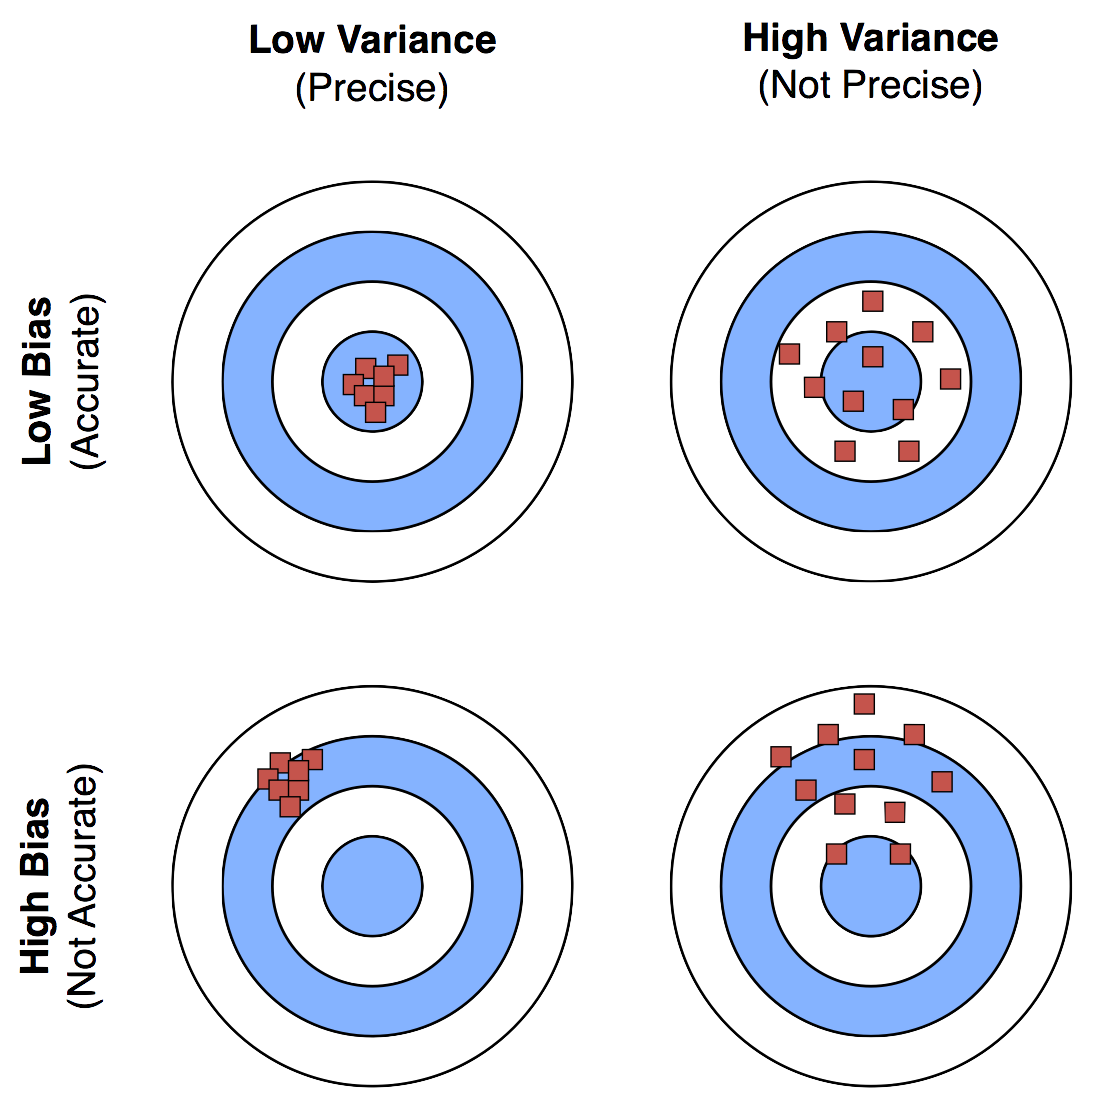
\includegraphics[width=60mm]{lecture5_g2}
\end{center}
\end{frame}

%%%%%%%%%%%%%%
\begin{frame}{The Bias/Variance Trade-off} 
\begin{center}
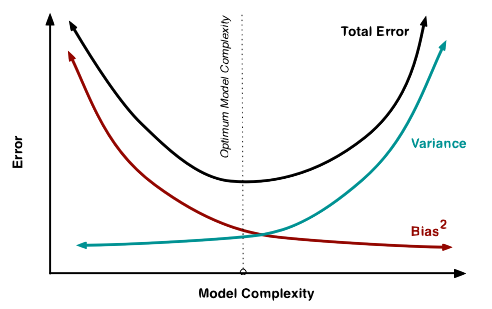
\includegraphics[width=60mm]{lecture5_g3}
\end{center}
\end{frame}

%%%%%%%%%%%%%%%%%%%%%%%%%%%%%%%%%%%%%%%%%%%%%%%%%%%%%%%%%%%%%%%%%%%%%%%%%%%%%%
\section{Regularization Methods: A Comparison}

%%%%%%%%%%%%%%
\begin{frame}{The Geometry of Regularization} 
\begin{center}
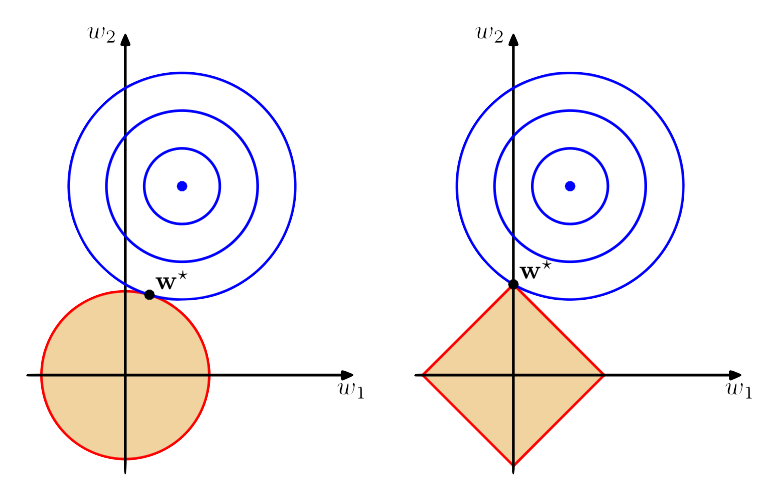
\includegraphics[width=100mm]{lecture5_g1}
\end{center}
\end{frame}

%%%%%%%%%%%%%%
\begin{frame}{Variable Selection as Regularization} 
Since LASSO regression tend to produce zero estimates for a number of model parameters - we say that LASSO solutions are \emph{sparse} - we consider LASSO to be a method for variable selection.
\vskip0.4cm
Many prefer using LASSO for variable selection (as well as for suppressing extreme parameter values) rather than stepwise selection, as LASSO avoids the statistic problems that arises in stepwise selection.
\end{frame}

%%%%%%%%%%%%%%
\begin{frame}{An Comparative Example} 

\end{frame}







%%%%%%%%%%%%%%%%%%%%%%%%%%%%%%%%%%%%%%%%%%%%%%%%%%%%%%%%%%%%%%%%%%%%%%%%%%%%%%
\begin{frame}{Bibliography}

\begin{enumerate}
 \fontsize{8}{10}\selectfont
\item Bolelli, L., Ertekin, S., and Giles, C. L. \emph{Topic and trend detection in text collections using latent dirichlet allocation}. In European Conference on Information Retrieval (2009), Springer, pp. 776-780.
\item Chen, W., Wang, Y., and Yang, S. \emph{Efficient influence maximization in social networks. In Proceedings of the 15th ACM SIGKDD international conference on Knowledge discovery and data mining (2009)}, ACM, pp. 199-208.
\item Chong, W., Blei, D., and Li, F.-F. \emph{Simultaneous image classification and annotation. In Computer Vision and Pattern Recognition}, 2009. CVPR 2009. IEEE Conference on (2009), IEEE, pp. 1903-1910.
\item Du, L., Ren, L., Carin, L., and Dunson, D. B. \emph{A bayesian model for simultaneous image clustering, annotation and object segmentation}. In Advances in neural information processing systems (2009), pp. 486-494.
\item Elango, P. K., and Jayaraman, K. \emph{Clustering images using the latent dirichlet allocation model.}
\item Feng, Y., and Lapata, M. \emph{Topic models for image annotation and text illustration}. In Human Language Technologies: The 2010 Annual Conference of the North American Chapter of the Association for Computational Linguistics (2010), Association for Computational Linguistics, pp. 831-839.
\item Hannah, L. A., and Wallach, H. M. \emph{Summarizing topics: From word lists to phrases.}
\item Lu, R., and Yang, Q. \emph{Trend analysis of news topics on twitter}. International Journal of Machine Learning and Computing 2, 3 (2012), 327.
\end{enumerate}

\end{frame}

\end{document}
